\documentclass[linenumbers]{aastex631}
\usepackage{graphicx}
\newcommand{\vdag}{(v)^\dagger}
\newcommand\aastex{AAS\TeX}
\newcommand\latex{La\TeX}

\begin{document}

\title{ASTR400B Research Proposal}

\author{Peter Hartman}
\affiliation{University of Arizona}

\section{Introduction} \label{sec:intro}
I propose to study the topic of the dark matter halo evolution of the M31/Milky Way Merger remnant, and particularly the density profile and kinematics of the dark matter halo.

Due to dark matter's purely gravitational interaction with baryons, its density profile is the most important component of dark matter's effect on galaxy evolution. The density profile of the halo is critical for the baryonic matter within the halo, as it determines the rotation rate of the galaxy and provides much of the mass to bind it. As such, the galactic structures we see heavily depend on the dark matter halo that they are embedded in.

While it is commonly understood that halos are well-fit by an NFW profile, there are still open questions about the halos, especially how they change. Questions of how the halo reacts to baryonic matter and how galaxy mergers alter the distribution of dark matter remain. Furthermore, there are still open questions on how the specific kinematics of dark matter halos affect merger remnants.

\cite{Abadi} showed that the dark matter halo reacts and changes shape due to the baryonic matter it influences. Inside of stellar mergers, these effects become very important, as a large amount of baryonic matter is interacting with both halos, affecting their density profiles.

\cite{DrakosA} found that the energy and spin parameters of the merging halos affect the remnant's halo distribution, with the spin parameter of the halo scaling linearly with the $c/b$ axis ratio and the energy parameter scaling with the $c/a$. The energy parameter also shows a relationship with the size of the resulting halo, as seen in Figure \ref{fig:1}. These factors provide a strong relationship between halo kinematics and the merger remnant halo properties.

\begin{figure}[h!]
    \centering
    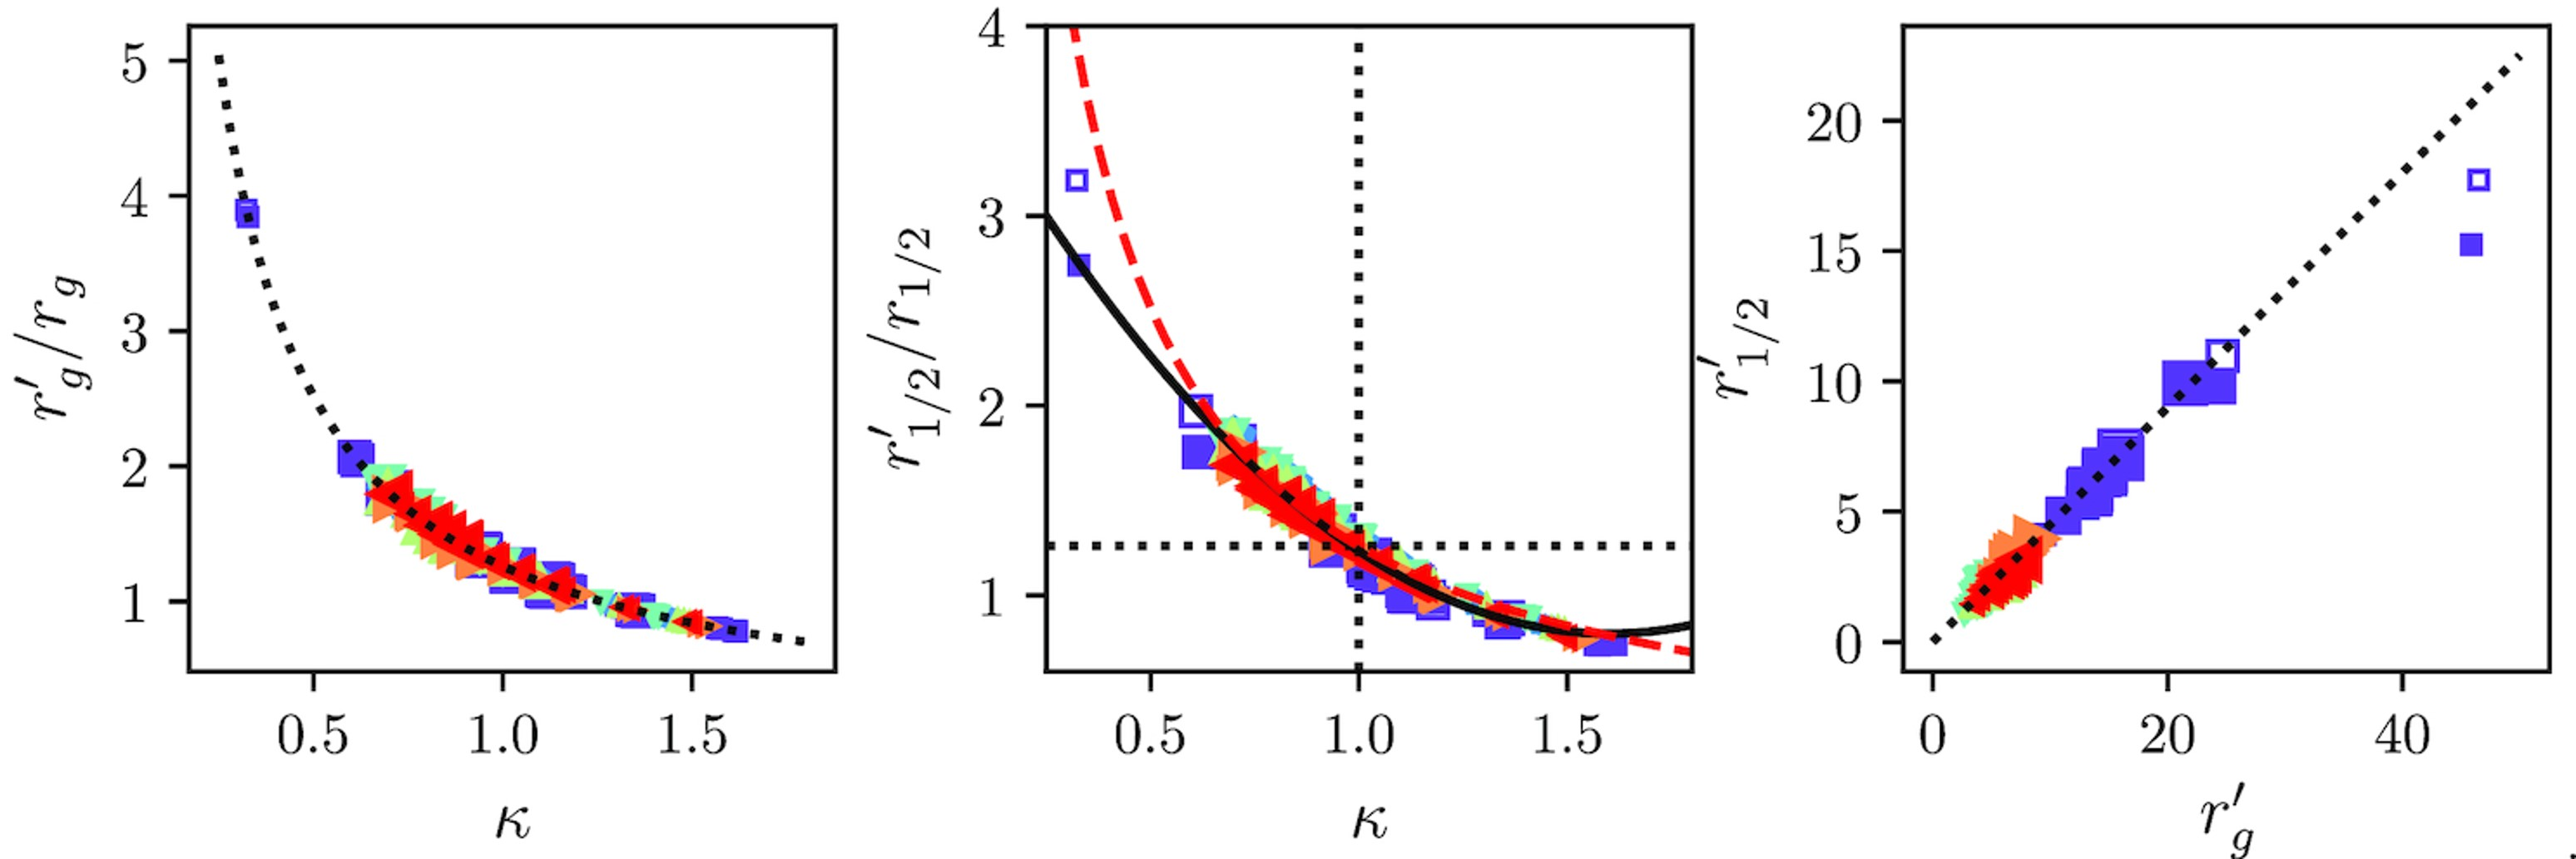
\includegraphics[width=\textwidth]{Drakos2019bFig7.jpg}
    \caption{(Left)The relationship between initial and final gravitational radius and the energy parameter $\kappa$. (Center) The relationship between initial and final half-mass radius and $\kappa$. (Right) The relationship between the gravitational radius and the half-mass radius. Each color corresponds to different types of halo profiles. We will not be testing these factors. Figure from \cite{DrakosB}}
    \label{fig:1}
\end{figure}
\newpage
\section{Proposal}

I will be addressing two questions. First, I will be studying the final dark matter density distribution after the merger. Second, I will be studying the kinematics of the halo after the merger. Both of these questions will rely on studying the difference between the initial and final conditions. In both cases, I will need to write new codes to find the energy and spin parameters in both states, as well as to determine if the Virial Theorem holds at different timesteps. The very general process is shown in \ref{fig:2}.
\subsection{Density Distribution}
I will be addressing the density profile by utilizing codes we have used in class already to collect information on the system as the merger continues and compare the initial density distribution of each galaxy's halo and the final merger halo. I will use our code from homework 6 to determine the time the merger completes, then write code to compare the initial halos and the final remnant halo. The primary parameter to compare here is the density distribution as a function of radius in each of the 3 spatial directions to determine the way the profile changes.

I expect that the remnant halo will be more massive and no longer spherically symmetric due to the merger. This is due to the relationship between the energy and spin parameters and final halo shape seen by \cite{DrakosB}. This means that it will no longer be well-fit by a Hernquist profile.

\subsection{Halo Kinematics}
I will be studying the kinematics of the merger by writing code to analyze the way kinematic motion changes between the initial and final halos. I will compare the motions of each galaxy halo relative to their center of the mass. I will write code to compute the dispersion of each galaxy given the simulation data, and determine if the virial theorem gives the right mass using another new code.

I expect that the merger remnant halo dispersion will depend on the spatial position asymmetrically (i.e. $\sigma_x \neq \sigma_y \neq \sigma_z$), as the halo will no longer be spherically symmetric. I expect the virial theorem to not provide the correct mass until a significant time after the galaxies merge, but to become correct as the system relaxes with time.

\begin{figure}[h]
    \centering
    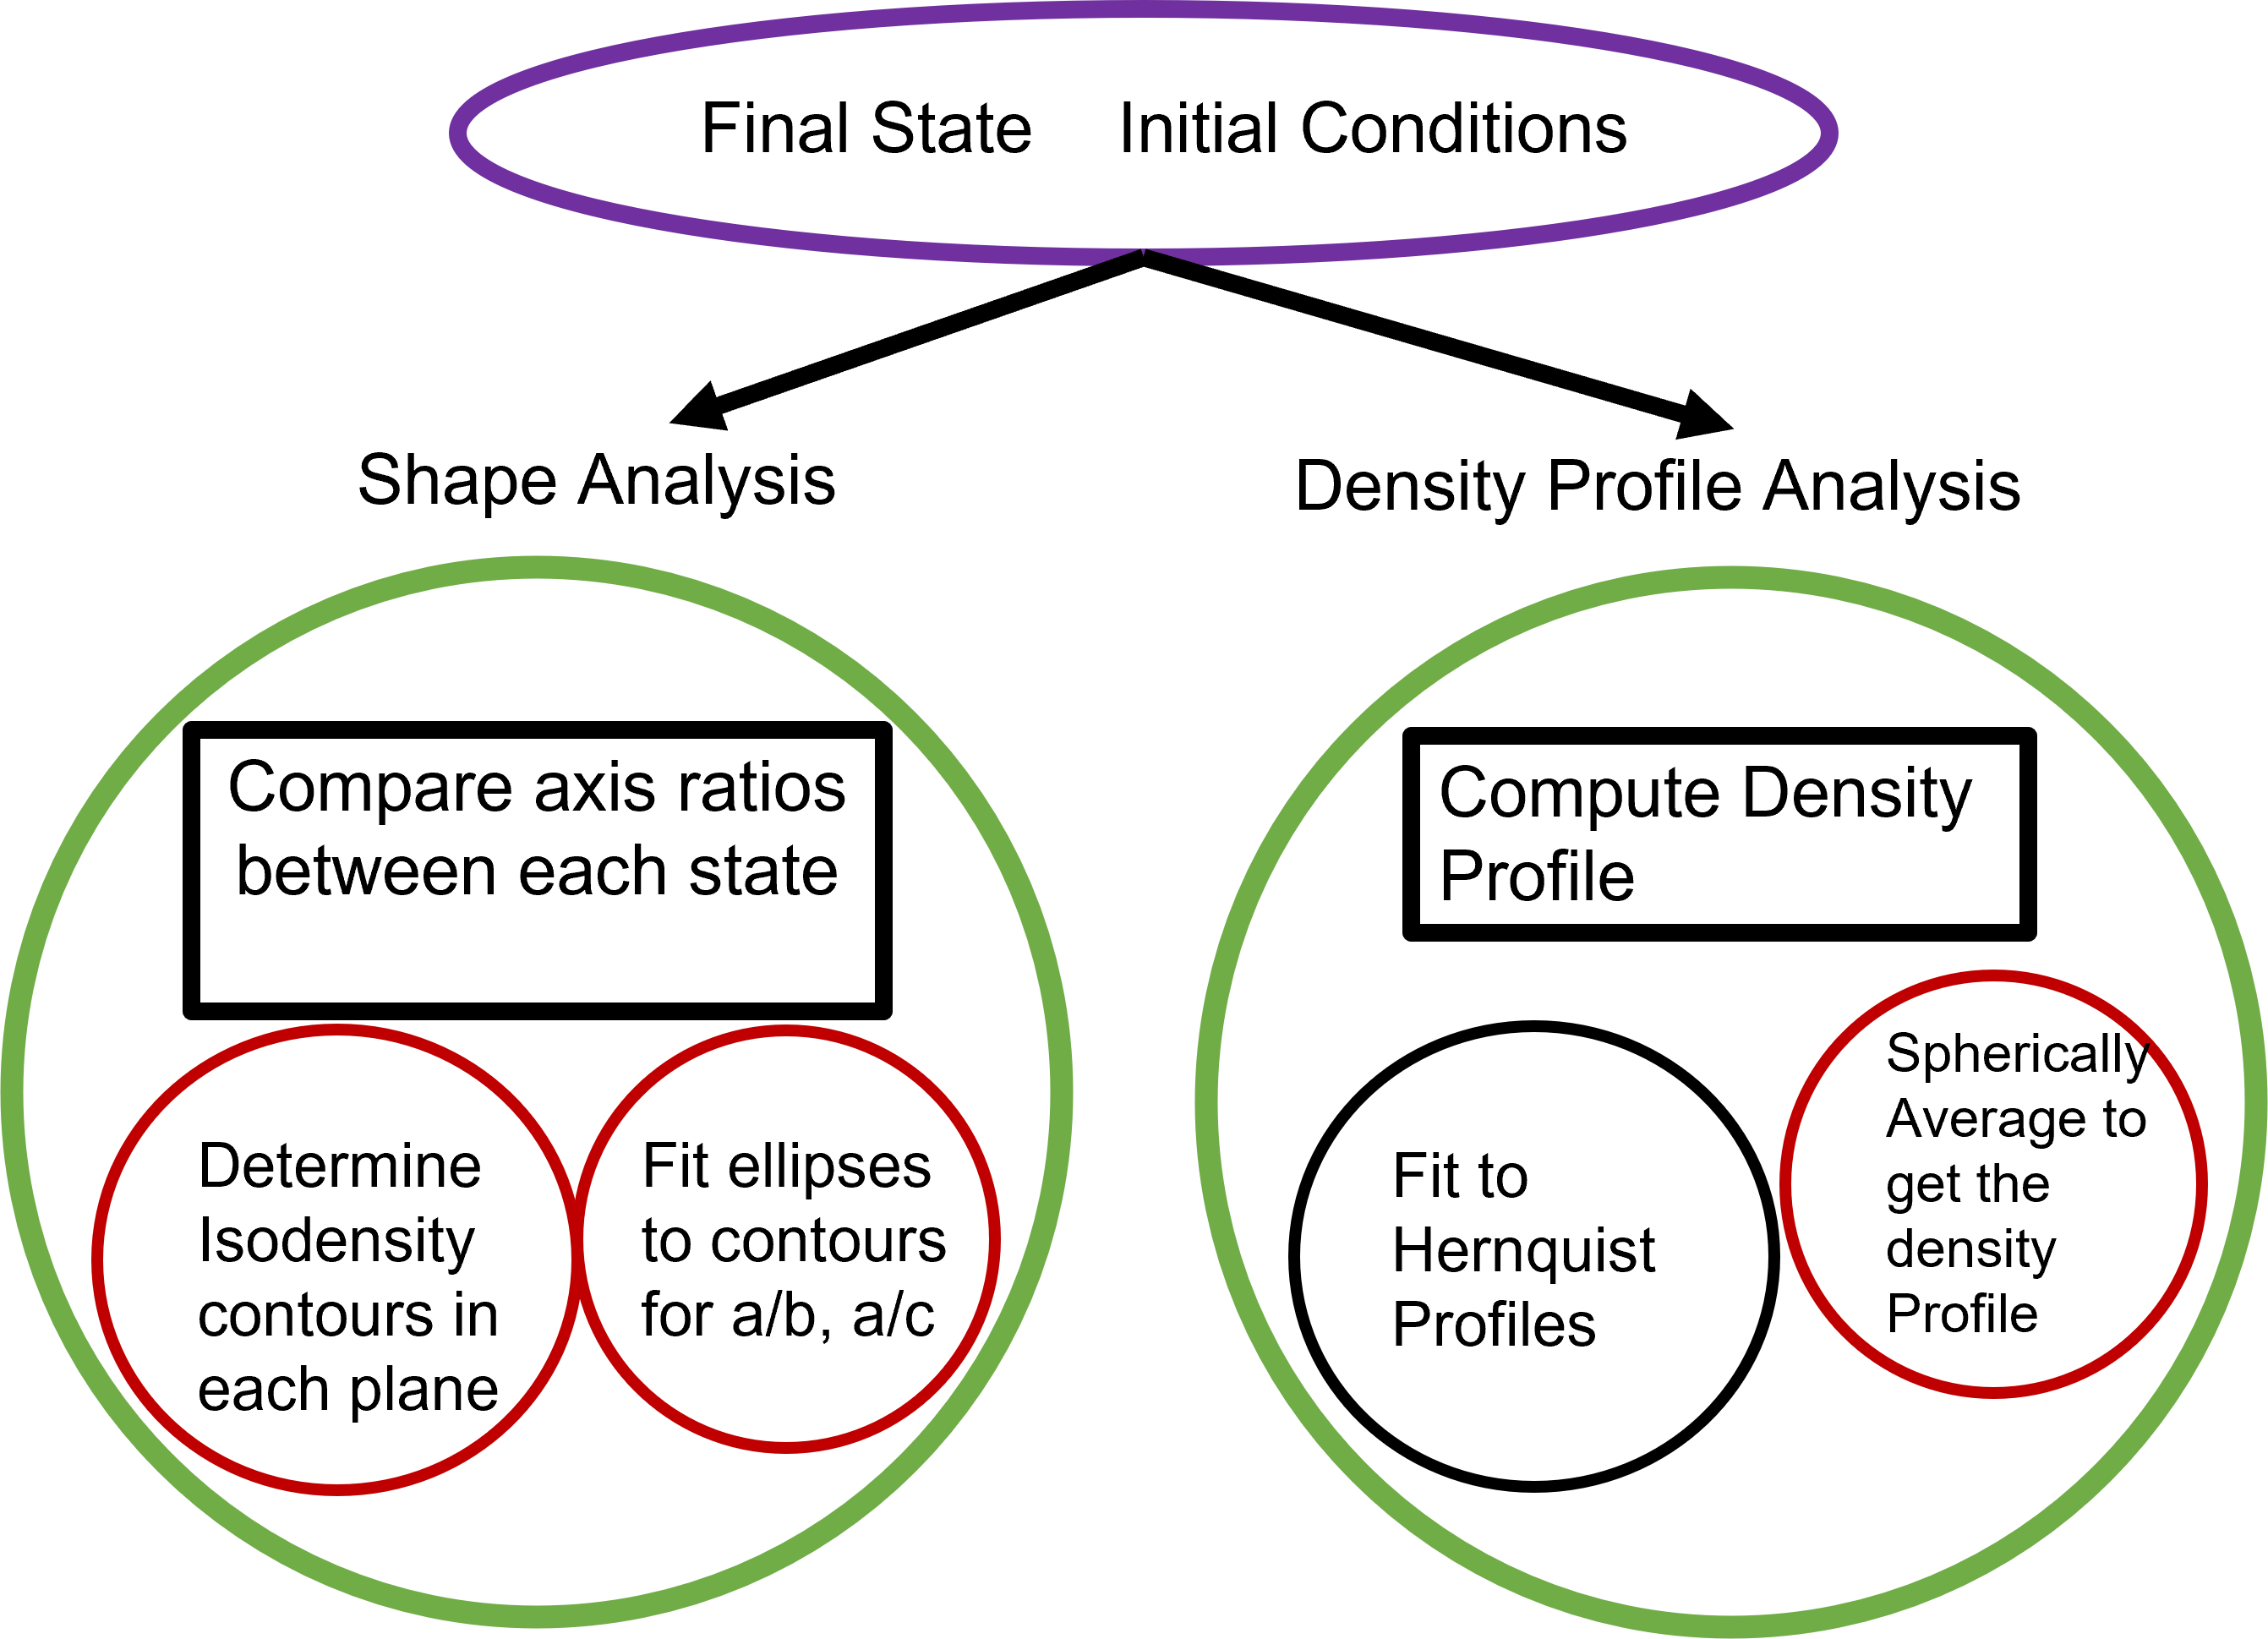
\includegraphics{MethodsFlowchart400B.png}
    \caption{A general overview of my process for analysis. The black borders indicate steps that will not require new codes, the red borders indicate the steps that will require new codes, and the green border indicates the step that will be the bulk of the analyzing of the data.}
    \label{fig:2}
\end{figure}

\bibliography{sample631}

\end{document}